\documentclass{beamer}
\RequirePackage[style=ieee]{biblatex}
\bibliography{../listings/bibliography}


\usetheme{Dresden}
\title{Ermöglichung des Hardware- und Software-in-the-Loop durch die Einbindung von BaSyx und MATLAB/Simulink}
\subtitle{Aktueller Zustand - April}
\author{Mateus Molina}
\institute{Technische Universität Kaiserslautern}
\date{\today}




\begin{document}

\begin{frame}
\titlepage
\end{frame}

\begin{frame}
    \frametitle{Outline}
    \tableofcontents
\end{frame}

\section{Zusammenfassung der abgearbeiteten Punkte}

\subsection{Theoretische Grundlagen}
\begin{frame}
    \frametitle{Theoretische Grundlagen}
    \begin{itemize}
        \item Simulationsprozess
        \begin{itemize}
            \item Hardware-in-the-Loop
            \item Software-in-the-Loop
        \end{itemize}
        \item MATLAB/Simulink und MBSE
        \begin{itemize}
            \item Model-Based Systems Engineering
            \item Simulink
            \item MATLAB S-Functions
        \end{itemize}    
        \item Industrie 4.0
        \begin{itemize}
            \item BaSys
            \item Eclipse BaSyx
                \begin{itemize}
                    \item digitaler Zwilling (AAS)
                    \item BaSyx-Komponenten
                \end{itemize}
        \end{itemize}    
        \item REST-Schnittstelle
    \end{itemize}
\end{frame}
\begin{frame}
    \frametitle{Simulationsprozess}
    \begin{itemize}
        \item \textbf{Hardware-in-the-Loop} Ein reales System durch Einsatz von physischen Prototypen ist oftmals wegen den mehreren Konfigurationsmöglichkeiten nicht möglich. Eine Alternative dazu stellt die Anbindung der Hardware an die Simulationsumgebung durch eine elektrische Schnittstelle \cite{zimmerDurchgangigerSimulationsprozessZur2015}
        \item \textbf{Software-in-the-Loop} Alternative für das Testen in früheren Phasen ist die Erstellung einer Software-Darstellung des Systems, die, die für die Phase notwendigen Anforderungen abdeckt.
    \end{itemize}
\end{frame}
\begin{frame}
    \frametitle{BaSys und BaSyx}
    \begin{itemize}
        \item \textbf{BaSys} Plattform-unabhängiges System, um die Grundlagen einer Produktionsanlage modellieren zu können \cite{chourtsidisScopingIndustryReconfigurability2020}
        \item \textbf{BaSyx} Open-Source-Referenzimplementierung von BaSys 4.0 und stellt SDK in verschiedenen Programmiersprachen zur Verfügung \cite{eclipsefoundationinc.BaSyxEclipsepedia}
    \end{itemize}
\end{frame}
\begin{frame}
    \frametitle{BaSyx}
    \begin{figure}[H]\centering
        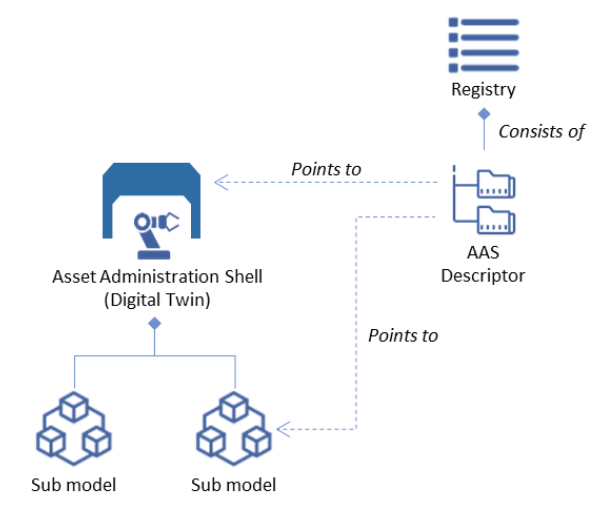
\includegraphics[width=10cm,height=5cm,keepaspectratio]{../media/2022-04-02-11-50-56.png}
        \caption{Diagramm einer Eclipse BaSyx-Systemstruktur (\cite{eclipsefoundationinc.BaSyxEclipsepedia})}
        \label{fig:basyxstruktur}
    \end{figure}
\end{frame}

\begin{frame}
    \frametitle{BaSyx-Komponenten}
    \begin{itemize}
        \item \textbf{AAS (digitaler Zwilling)} stellt das digitale Abbild eines physischen Gegenstands und die Schnittstelle für die Kommunikation in der digitalen Umgebung dar \cite{plattformindustrie4.0DiskussionspapierVerwaltungsschalePraxis}
        \item \textbf{Submodel} Datenmodelle, die bestimmte Aspekte einer Anlage beschreiben, z. B. ihr digitales Typenschild, die angebotenen Dienstleistungen oder die Anlagentopologie \cite{eclipsefoundationinc.BaSyxEclipsepedia}
        \item \textbf{VAB}  ermöglicht die direkte Kommunikation über die verschiedenen Schichten der Automatisierungsstruktur \cite{fraunhofer-institutfurexperimentellessoftwareengineeringieseBaSysFlyer}
        \item \textbf{Registry} ermöglicht die Registrierung und Suche von AAS innerhalb definierter Systemgrenzen \cite{eclipsefoundationinc.BaSyxEclipsepedia}
    \end{itemize}
\end{frame}
\begin{frame}
    \frametitle{Simulink}
    \begin{itemize}
        \item \textbf{S-Function} eine in einer der unterstützten Programmiersprachen von MATLAB (MATLAB, C, C++ oder Fortran) geschriebene Beschreibung eines Simulink-Blocks in Computersprache  \cite{themathworksinc.WhatSFunctionMATLAB}.
    \end{itemize}
\end{frame}
\begin{frame}
    \frametitle{REST-Schnittstelle}
    \begin{itemize}
        \item \textbf{REST} am meisten verbreitete Kommunikationsarchitektur zur Vernetzung von Maschinen und wird bei mehreren Anwendungsfällen angewandt, wie z.B. IoT-Technologien \cite{reinheimerIndustrieHerausforderungenKonzepte2017}
    \end{itemize}
\end{frame}


\subsection{Einleitung}
\begin{frame}
    \frametitle{Motivation}
    \begin{itemize}
        \item Simulink zusammen mit BaSyx könnten eingesetzt werden, um \emph{Hardware-In-The-Loop}, bzw. \emph{Software-In-The-Loop} leichter einzusetzen, wobei BaSyx um die Struktur der digitalen Zwillinge kümmern würde, während Simulink für das Simulieren einzelner Bauteile oder Regelung gesamter Komponenten angewandt würde.
        \item Nach Prüfung von verschiedenen Alternativen, Simulink und BaSyx zusammen einzusetzen, hat sich herausgestellt, dass eine Kommunikationsschnittstele zusätzliche Kenntnisse im C, REST und die innere Funktionsweise vom BaSyx voraussetzt, was ein limitierender Faktor für eine breitere Verwendung in der Industrie darstellen könnte.
    \end{itemize}
\end{frame}

\begin{frame}
    \frametitle{Motivation}
    Eine unkomplizierte und erfolgreiche Verbindung der beiden Plattformen würde dem Stand der Technik folgende Vorteile bringen:
    \begin{itemize}
        \item Mehr Anreiz, früher im Projekt nach BaSys strukturierte digitale Zwillinge einzusetzen
        \item vereinfachte und schnellere Anbindung eines zu testen Hardware/Software an ein MATLAB/Simulink-Modell;
        \item Reduzieren der Lernkurve, Ingenieure in Simulink mit BaSyx verträglichen Modellen herstellen zu können;
        \item wirksame Einsetzung realer Daten in MATLAB/Simulink/Modellen.  
    \end{itemize}

\end{frame}
\begin{frame}
    \frametitle{Zielstellung}
    \begin{enumerate}
        \item Entwicklung einer Bibliothek für MATLAB/Simulink, um die Verbindung mit BaSyx AAS zu vereinfachen;
        \item Einsetzung der Bibliothek in einem Anwendungsbeispiel.
    \end{enumerate}    
\end{frame}


\subsection{Referenzen}

\begin{frame}[allowframebreaks]
    \frametitle{Referenzen für diese Präsentation}
    \printbibliography

\end{frame}

\section{Diskussion}
\begin{frame}
    \frametitle{Verteilung erstes Entwurfes}
    Der erste Entwurf der Projektarbeit wird am Ende des Meetings verteilt. 
\end{frame}

\begin{frame}
    \frametitle{Diskussion}
    \begin{enumerate}
        \item Umfang und Datum der nächsten Abgabe
        \item Notwendigkeit einer Machbarkeitsstudie
        \item Marktforschung, um das Projekt zu rechtfertigen. Wie könnte ich es am besten durchführen?
    \end{enumerate}

\end{frame}

\end{document}